\section{Software}
Die Steuerung der Segel soll durch zwei verteilte Systeme erfolgen, die über eine Ethernet-Verbindung miteinander kommunizieren. Die Idee dahinter ist, die Berechnungen für die Ausrichtung der Segel in Abhängigkeit der Windstärke und -Richtung (Controllino) von der hardwarenahen Verarbeitung der Sensoren und Aktuatoren (stm32) logisch zu trennen. \\
Die vorliegende Arbeit konzentriert sich dabei lediglich auf das System der Sensoren und Aktuatoren, welches mit dem stm32 realisiert wurde. Die Aufgabe dieses Systems ist, zunächst die Linearführung zu kalibrieren, damit die aktuelle Position korrekt ermittelt werden kann. Außerdem soll über die Buttons am Gehäuse und zusätzlich über einen Webserver eine manuelle Steuerung ermöglicht werden. Während des Automatikbetriebs geschieht ein regelmäßiger Austausch aller relevanter Daten über eine REST basierte Schnittstelle. Dies beinhaltet u.A. die Information über aktuelle Windbedingung, Position der Segel, eventuelle Fehlerzustände (z.B. Motorfehler oder Überstrom) und daraus resultierende Befehle zur Anpassung der Segelstellung.
Für die Implementierung wurde die Software in komponentenorientierte Module eingeteilt:

\begin{figure}[h]
	\centering
	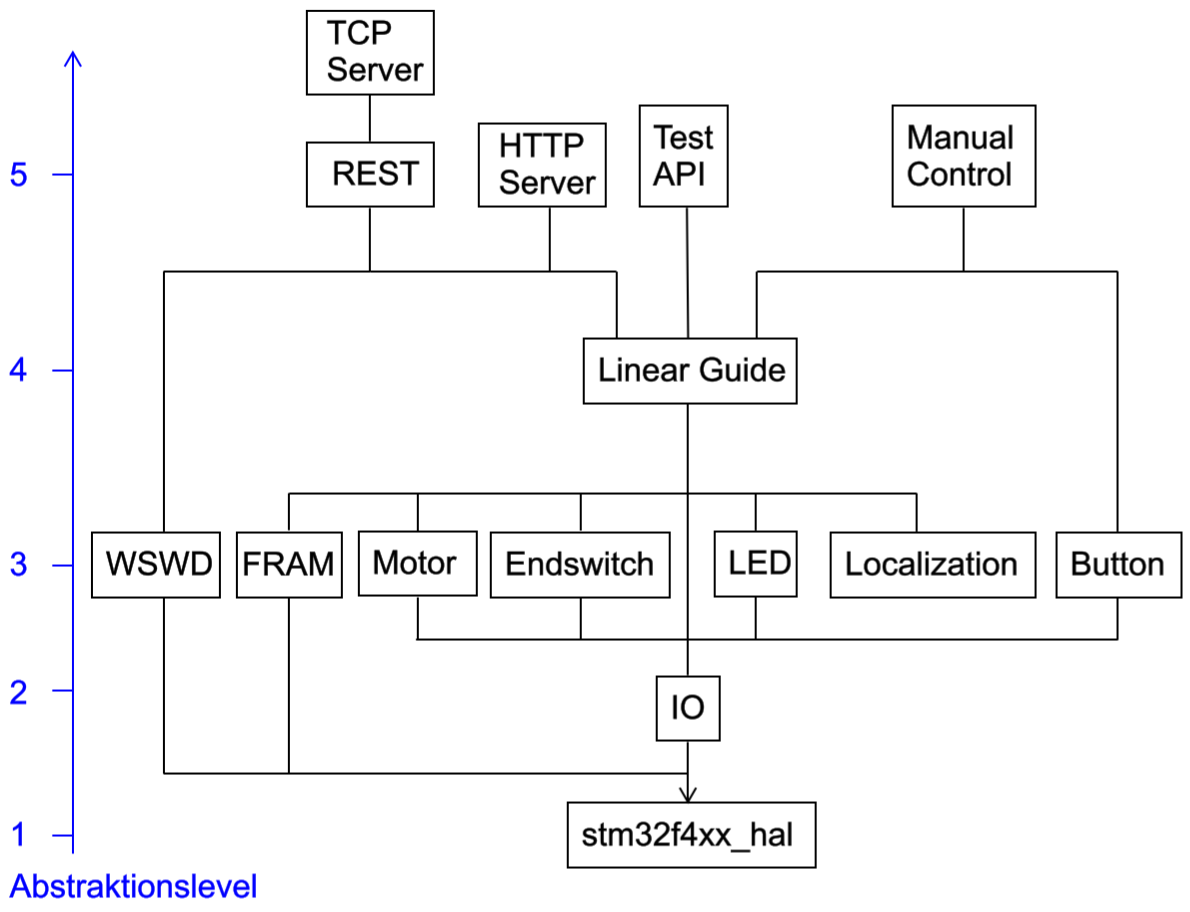
\includegraphics[width=0.6\linewidth]{images/Software/Modulestructure.png}
	\caption{Software Modulstruktur}
	\label{fig:modulestructure}
\end{figure}
\noindent
Abbildung \ref{fig:modulestructure} zeigt abwärtsgerichtet, wie die einzelnen Module aufeinander zugreifen. Auf unterster Abstraktionsebene laufen jegliche Operationen über die Standardbibliothek des Mikrocontrollers \texttt{stm32f4xx\_hal}. Darüber liefert das \texttt{IO}-Modul ein Set aus Hilfsfunktionen und -Strukturen für den allgemeinen Zugriff auf die GPIO-Pins und zum Auslesen analoger Messwerte der einzelnen Sensoren. Ebene 3 umfasst hauptsächlich Module, welche alle relevanten Funktionalitäten der physischen Teilkomponenten des Systems implementieren, wie z.B. das Anemometer \texttt{WSWD} oder der \texttt{Motor}. Einige davon greifen dabei auf das \texttt{IO}-Modul zu, wobei der allgemeine GPIO-Zugriff von einer spezifischen Funktion eingekapselt wird, wie z.B. das Einschalten einer LED im Falle des \texttt{LED-Moduls}. Eine Ausnahme ist das \texttt{Localization}-Modul, welches keine physische Komponente darstellt, sondern einige Hilfsfunktionen zur Kalibrierung und Positionsberechnung bereitstellt. Während die Module bis Ebene 3 überwiegend allgemeingültig entworfen sind, enthält das \texttt{Linear Guide}-Modul anwendungsspezifische Funktionen. Als zentrales Element bildet dieses ein High-Level Interface zur Verwendung der Teilkomponenten \texttt{FRAM}, \texttt{Motor}, \texttt{Endswitch}, \texttt{LED}, \texttt{Localization} und \texttt{IO}. Die Module der obersten Abstraktionsebene bilden die direkten Schnittstellen zur Außenwelt. Das \texttt{Manual Control}-Modul ermöglicht die manuelle Steuerung der Linearführung über die User-Buttons am Gehäuse und insbesondere die Umsetzung des Kalibrierungsprozesses. Auf der anderen Seite kann das System auch durch ein HTTP Webserver überwacht und gesteuert werden. Zuletzt werden im \texttt{REST}-Modul die Anfragen des Controllinos über die \texttt{TCP Server}-Verbindung verarbeitet, wie bereits oben erwähnt.
